\documentclass[ams, a4j]{U-AizuGT}
\usepackage{pifont}
% \usepackage{graphicx}
\usepackage{cite}
\usepackage{mathtools}
% \usepackage{listings,jvlisting}
% \documentclass[a4j]{jarticle} %ここは関係ない
\usepackage{listings,jvlisting} 
\usepackage[dvipdfmx]{graphicx}
\lstset{
    frame=single,
    numbers=left,
    tabsize=2
}


% \usepackage{listings,jlisting}

% \lstset{%
%   language={C},
%   basicstyle={\small},%
%   identifierstyle={\small},%
%   commentstyle={\small\itshape},%
%   keywordstyle={\small\bfseries},%
%   ndkeywordstyle={\small},%
%   stringstyle={\small\ttfamily},
%   frame={tb},
%   breaklines=true,
%   columns=[l]{fullflexible},%
%   numbers=left,%
%   xrightmargin=0zw,%
%   xleftmargin=3zw,%
%   numberstyle={\scriptsize},%
%   stepnumber=1,
%   numbersep=1zw,%
%   lineskip=-0.5ex%
% }
\lstset{
  basicstyle={\ttfamily},
  identifierstyle={\small},
  commentstyle={\smallitshape},
  keywordstyle={\small\bfseries},
  ndkeywordstyle={\small},
  stringstyle={\small\ttfamily},
  frame={tb},
  breaklines=true,
  columns=[l]{fullflexible},
  numbers=left,
  xrightmargin=0zw,
  xleftmargin=3zw,
  numberstyle={\scriptsize},
  stepnumber=1,
  numbersep=1zw,
  lineskip=-0.5ex
}

\bibliographystyle{ieice}
\author{Ryuki Hiwada}
\studentid{s1280076}
\supervisor{Naohito Nakasato}

\title{Domain Specific Language for high performance computing}

\begin{document}
\maketitle
\begin{abstract}

\end{abstract}
\section{Introduction}


\subsection{Background}
In astrophysics and astronomy, to numerically calculate the dynamical 
evolution of N particles interacting gravitationally, N-body simulations 
are required. Figure 1 shows the equation for interparticle interactions 
in N-body simulations. If the equation is naively computed, the time
complexity of calculation of interparticle interactions is 
\begin{math}O(N^2) \end{math}, where 
N is the number of particles. Therefore, parallelization is required to
speed up numerical simulations. To write a parallelized code for a 
numerical simulation, a user needs to understand the architecture of 
computer systems in  detail. If a parallelized code is automatically
generated by only describing the formulas and data of the numerical
simulation, the above problems are solved. To realize the parallelization,
we will develop Domain Specific Language  DSL \rparen, which is a 
programming language specialized to a domain, for example, SQL and HTML.
\subsection{parallelization}
SIMD is one of the categories in Flynn's taxonomy 1, related to computer arithmetic
 processing. Using SIMD, arithmetic operations can be applied simultaneously to
multiple data. In this paper, we compute and parallelize multiple particles. For example, 
as shown in Figure 1, the computation of acceleration for different particles is independent
of each other, allowing the process to be parallelized. As a result, for instance Assuming 
that the variables for particles are double-precision floating-point numbers, we can execute 
an operation on four elements simultaneously using the AVX2 instruction, it is possible to 
perform operations on four elements. Therefore, compared to non-parallelized code, there is
a potential to accelerate the computation by four times. We will describe the design of a 
DSL in the next section to generate such parallelized code from the formulation of particle-particle interactions.
\subsection{Overview of DSL}

We have created a Domain Specific Language  DSL \rparen named  Pyker \rparen. This language's 
processor can read code describing particle interaction formulas and generate code 
that accelerates these computations. The language allows for the definition of 
variables and the description of interaction formulas. In the variable definition 
section, it's possible to define variables such as the mass and position of 
particles, variables for storing results, and other necessary variables. For the formula
part, we have enabled calculations including basic arithmetic operations, sqrt, power 
functions, and computing the norm of vectors. From this description, a kernel function 
is generated, which can then be called and used. We have created a Domain Specific 
Language  DSL  named  Pyker. This language's processor can read code describing particle 
interaction formulas and generate code that accelerates these computations. The language allows
for the definition of variables and the description of interaction formulas. In the variable
definition section, it's possible to define variables such as the mass and position of 
particles, variables for storing results, and other necessary variables. For the formula part, 
we have enabled calculations including basic arithmetic operations, sqrt, power functions, and 
computing the norm of vectors. From this description, a kernel function is generated, which can then be called and used.
\subsection{Aim of this paper}



\section{Construction}
We use Sympy, a library in Python for implementing  the implementation of pyker.
SymPy supports various operations, and the formulas using these operations are internally treated as 
syntax trees. We leveraged this functionality to read formulas and generate code capable of parallel execution.
For parallelization, we used an instruction set named Advanced Vector Extensions 2 \lparen AVX2\rparen. AVX2 is one of the 
extended instruction sets implemented in Intel's CPUs. The next section will explain how parallelization is carried out using AVX2.


\subsection{AVX2 for parallelization}
% _mm256dの説明はここですべきか? codegen で説明すべきか
To perform SIMD operations, just like with regular computations, data is first loaded from memory, computed based on that data,
and the results are stored. However, in the case of SIMD, computations are performed using SIMD-specific registers, so the 
methods of loading, computing, and storing differ. When loading, multiple elements that will undergo the same instruction are
stored in a SIMD-specific register. These are then used to perform computations simultaneously, and the results are stored for
each. 


For instance, consider a calculation like C = X + Y, where elements of double-precision floating arrays x and y are computed
. When using AVX2 for SIMD, since the registers are 256 bits, four elements from x and y are loaded each. These are then added 
simultaneously, and the results are stored in the array C. When loading into SIMD registers, if it's a 1-dimensional array, 
contiguous memory access is sufficient, but for data structures like Array of Structures \lparen AoS \rparen shown in Figure a., elements need
to be loaded individually. 


For example, when considering the 3-dimensional coordinates of particles as double-precision floats 
in pos\lbrack n\rbrack \lbrack 3\rbrack  \lparen where n is the total number of particles, and pos\lbrack i \rbrack \lbrack 0\rbrack , pos\lbrack i\rbrack \lbrack 1\rbrack , 
pos\lbrack i\rbrack \lbrack 2\rbrack  represent the x, y, z coordinates 
of the i-th particle, respectively\rparen, and calculating the difference in x coordinates between particles i and j, it becomes dx = 
pos\lbrack i\rbrack \lbrack 0\rbrack  - pos\lbrack j\rbrack \lbrack 0\rbrack . However, for parallelization with SIMD, desiring dx0 = pos\lbrack i\rbrack \lbrack 0\rbrack  - pos\lbrack j \rbrack \lbrack 0\rbrack , dx1 = pos\lbrack i+1\rbrack \lbrack 0\rbrack  - pos\lbrack j\rbrack \lbrack 0\rbrack 
, dx2 = pos\lbrack i+2\rbrack \lbrack 0\rbrack  - pos\lbrack j\rbrack \lbrack 0\rbrack , dx3 = pos\lbrack i+3\rbrack \lbrack 0\rbrack  - pos\lbrack j\rbrack \lbrack 0\rbrack , 
the data are packed as \lparen pos\lbrack i\rbrack \lbrack 0\rbrack , pos\lbrack i+1\rbrack \lbrack 0\rbrack , pos\lbrack i+2\rbrack \lbrack  0\rbrack , pos\lbrack  i+3\rbrack \lbrack  0\rbrack \rparen,
\lparen pos\lbrack  j\rbrack \lbrack  0\rbrack , pos\lbrack  j\rbrack \lbrack  0\rbrack , pos\lbrack  j\rbrack \lbrack  0\rbrack , pos\lbrack  j\rbrack \lbrack  0\rparen, \lparen dx0, dx1, dx2, dx3\rparen and subtraction is performed simultaneously. However, since data needs
to be loaded onto SIMD registers all at once, the gather instruction is used to load data for particle i. The gather instruction is used
to read non-contiguous data elements from memory addresses by specifying addresses. An explanation of the gather instruction is shown in 
Figure x. Data loaded in this way are computed simultaneously using SIMD instructions. 


When storing computation results, addresses may 
not be contiguous. In such cases, there is an instruction called scatter, which is the counterpart to gather, but it is not supported 
in AVX2, so data are stored using pointers individually. In this way, parallelization is achieved with SIMD. Moreover, these instructions
can be explicitly handled in high-level programming languages like C and C++ using intrinsic functions. To handle intrinsic functions 
in C and C++, include the file immintrin.h, which is available as a standard in the language. An example of C++ code that calculates the difference in x coordinates, simd\_tmp.cpp, is shown. { Pyker}  generates C++ code capable of executing SIMD instructions like simd\_tmp.cpp
from the described formulas. The next section will explain the Pyker.

\subsection{Pyker}
In this DSL, code is generated by writing and compiling two definitions: the definition of variables and the definition of interaction formulas. First, let us explain the variable definition.


In this DSL, variables are classified into classes: EPI, EPJ, FORCE, and others. EPI represents particles that receive interactions, 
while EPJ represents particles that provide interactions. FORCE holds the results of the interaction calculations, and other variables 
include softening parameters and the like. To perform calculations using these variables, in C++, it would be similar to \ref{fuga}.


\begin{lstlisting}[frame=single, caption=hoge, label=fuga]
int kernel(double xi[][3], double xj[][3], double ai[][3], double eps2, int n){
	// (1).preprocess
	for(int i = 0;i < n;i += 4) {
		// (2).load EPI 
		// (3).Initialization of tmporary force
		for(int j = 0;j < n;j += 1) {
				// (4). calculate interparticle interactions
		}
		// (5). Store calculation result in the FORCE
	}
}
\end{lstlisting}

(1) involves preparatory steps such as defining variables necessary for the calculation. (2) 
involves loading the variables of EPI. (3) is about initializing variables that temporarily
 hold the results of the interaction calculation. (4) involves performing the interaction 
 calculation and saving the results in the primary variable of force. (5) involves storing the results in the FORCE variables.
To generate this code, in variable definition, information about the class of the variable,
 its type, and its dimension is necessary. Therefore, in pyker, variable definitions are written as follows. .
The first column, if it is a class, writes the name of the class and its member variable
 name. The second column explicitly writes the dimensions of the vector if there are any, 
 specifying 3 or 4 dimensions, and the type is either 32-bit or 64-bit floating-point. The 
 third column becomes the name of the variable handled on pykg. For example, "EPI.pos vec3<F64> xi" 
 would be a member variable of EPI named pos, a 3-dimensional 64-bit floating-point variable named xi.
The definition of interaction formulas is written to accumulate the results in the FORCE variable using
 the defined variables. Primary variables necessary for the mathematical description can be newly defined 
 using previously defined variables. Available operations include basic arithmetic, sqrt, and the power 
 symbol "**". The result is stored in the FORCE variable using '='.For instance, to generate code that c
 alculates the gravitational interaction formula shown in Figure 1, it would be written in this DSL as figure1.pyker.


\begin{lstlisting}[frame=single, caption=hoge, label=fuga]
EPI.pos vec3<F64> xi
EPJ.pos vec3<F64> xj
EPJ.m F64 mass
FORCE.acc vec3<F64> ai
F64 eps2
F64 g
dr = xj - xi
ai = g * mass *  dr / sqrt(dr ** 2 + eps2) ** 3
\end{lstlisting}
\subsection{Implementation}
The process of generating code is illustrated in the following flowchart. In Parsing, the information
of the variables defined in the DSL code is converted into a hash with the variable names as keys. 
Formulas are converted into syntax trees using the sympify() method of Sympy, and a list of these 
trees is obtained. Next, Common Subexpression Elimination (CSE) is performed on the syntax trees of the converted formulas. CSE is the process 
of reducing the number of operations by pre-calculating common subexpressions in formulas and using 
their results in subsequent calculations. In type inference, the types of the primary variables in the 
formulas are inferred. Afterward, all syntax trees are converted into binary trees to align them with 
SIMD operations. Finally, the code for calculating interactions is generated by traversing the processed 
syntax trees. The following sections describe how the implementation was carried out in the order of
Parsing, CSE, type inference, conversion to binary trees, and Code generation.
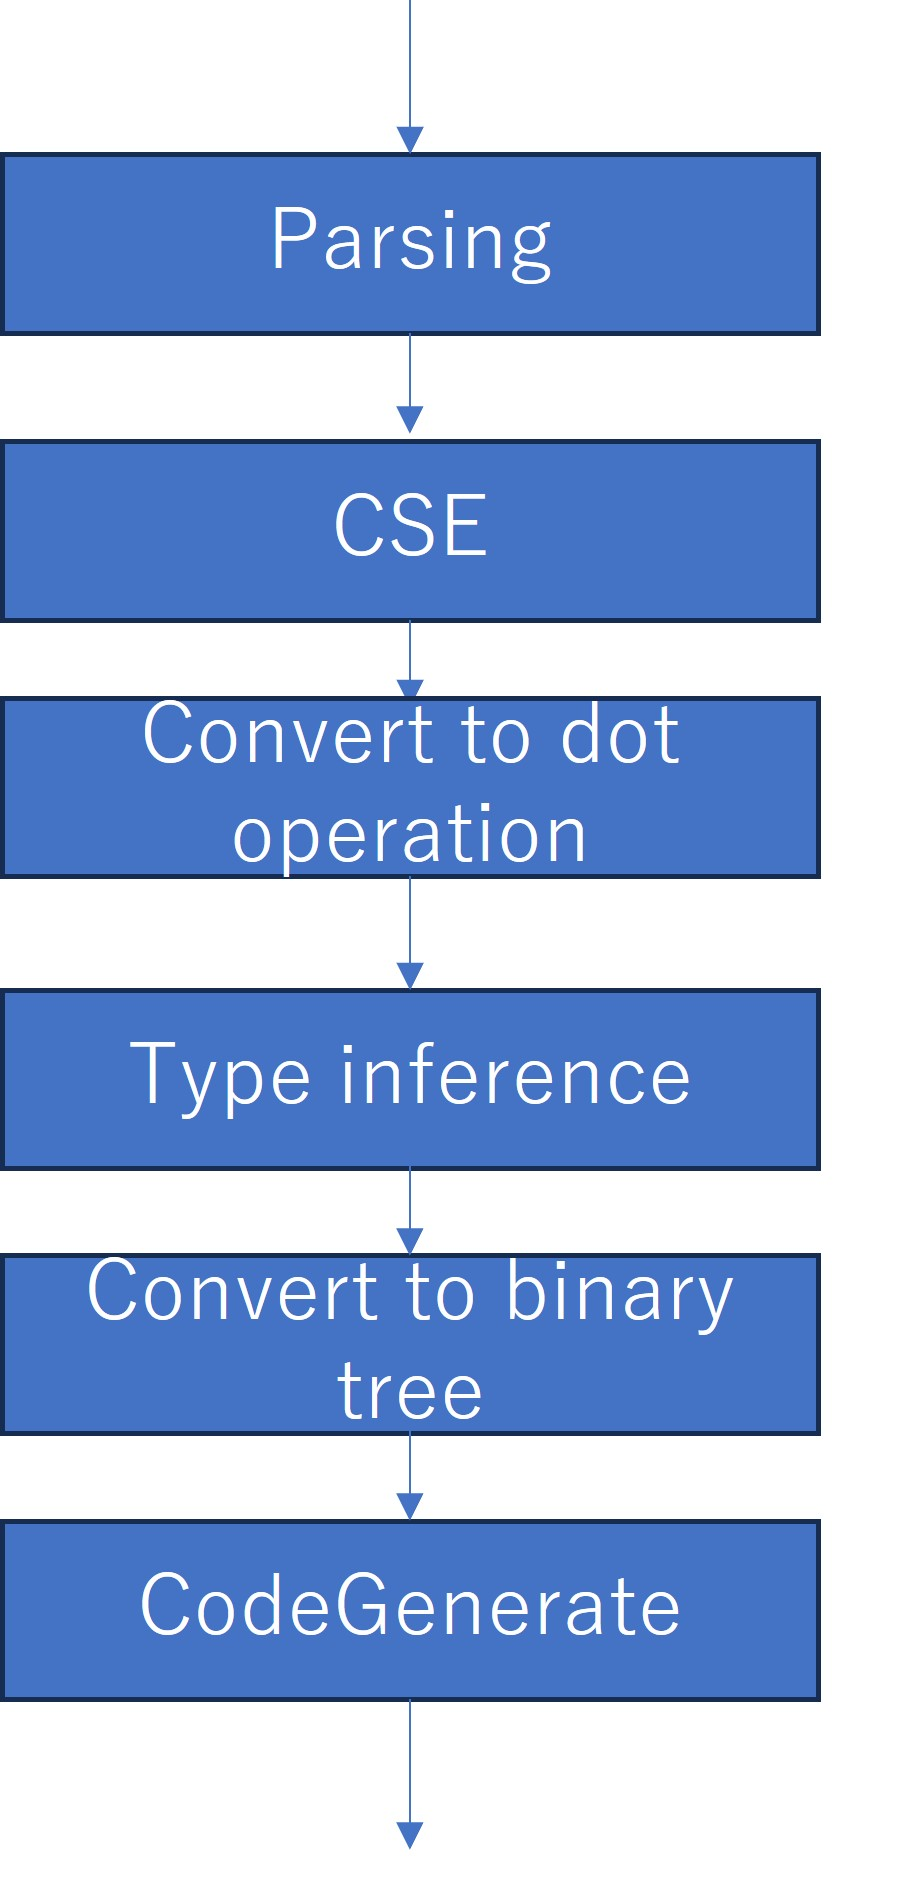
\includegraphics[width=0.2\textwidth]{flowchartver3.jpg}
\subsubsection{Parsing}
In Parsing, the process is divided between variable definition and formula handling. In variable definition, 
objects with class, vector, type, and variable name are created respectively. A hash with the variable name
as the key is then made (name\_variable\_map). Formulas use the sympify() method from the Sympy library to convert
the code read as a string into a syntax tree of formulas, obtaining a list of these syntax trees (expr\_list). Next, 
Common Subexpression Elimination (CSE) is performed.
\subsubsection{CSE}

\subsubsection{type inference}
\subsubsection{convert to binary trees}

\subsubsection{code generatation of non SIMD}

\begin{lstlisting}[frame=single, caption=hoge]

#include<math>
int kernel( (1) double xi[][3], double xj[][3], double eps2, double ai[][3], ...) {
  //(2)
  int i;
  int j;
  double dr_v0;
  double dr_v1;
  double dr_v2;
  // ... 
  // ... 
  // ... 

  for(i = 0;i < n;i += 1) {
    for(j = 0;j < n;j += 1) {
      //(3)
      dr_v0 = -xi[i][0] + xj[j][0];
      dr_v1 = -xi[i][1] + xj[j][1];
      dr_v2 = -xi[i][2] + xj[j][2];
      // ... 
      // ... 
      // ... 
    }
  }
}
\end{lstlisting}
  

\subsubsection{code generatation of SIMD}


\begin{lstlisting}[frame=single, caption=hoge]
//(1) include part
#include<math>
#include<immintrin.h>
int kernel( (2) double xi[][3], double xj[][3], double eps2, double ai[][3], ...) {
  //(3) decleare tmp variable
  int i;
  int j;
  __m256d xi_tmp_v0;
  __m256d xi_tmp_v1;  
  __m256d xi_tmp_v2;
  __m256d eps2_tmp;
  // ... 
  // ... 
  // ... 
  //(4) def not class variables
  eps2_tmp = _mm256_set1_pd(eps2);
  // ... 
  // ... 
  // ... 
  
  // (5) loop increment
  for(i = 0;i < n;i += 4) {
    // (6) Load EPI variable part
    int index_gather_0[4] = {0, 3, 6, 9};
    __m128i vindex_gather_0 = _mm_load_si128((const __m128i*)index_gather_0);    
    // ... 
    // ... 
    // ... 

    // (7) initialize result temporary variable
    ai_tmp_v0 = _mm256_set1_pd(0.0);
    ai_tmp_v1 = _mm256_set1_pd(0.0);
    ai_tmp_v2 = _mm256_set1_pd(0.0);


    for(j = 0;j < n;j += 1) {
      // (8) Load EPJ variable part
         xj_tmp_v0 = _mm256_set1_pd(xj[j][0]);
         xj_tmp_v1 = _mm256_set1_pd(xj[j][1]);
         xj_tmp_v2 = _mm256_set1_pd(xj[j][2]);
        // ... 
        // ... 
        // ... 
         

      // (9) calculate interparticle
        dr_tmp_v0 = _mm256_sub_pd(xj_tmp_v0, xi_tmp_v0);
        dr_tmp_v1 = _mm256_sub_pd(xj_tmp_v1, xi_tmp_v1);
        dr_tmp_v2 = _mm256_sub_pd(xj_tmp_v2, xi_tmp_v2);
        ai_tmp_v0 += _mm256_div_pd(_mm256_mul_pd(//.....));
        ai_tmp_v1 += _mm256_div_pd(_mm256_mul_pd(//.....));
        ai_tmp_v2 += _mm256_div_pd(_mm256_mul_pd(//.....));

    }

    // (10) Store result part

  }
  return 0;
}
\end{lstlisting}



\section{Experiments}

\section{Conclusion}
\section{Acknowledgement}
\bibliography{biblist}
\end{document}